This fact has the following consequence. \lesson{23}{30/04/2020}
\begin{proposition}[Defaultable bond]
    The down-and-out bond with barrier $L$ is priced by the formula
    \begin{equation}
        BO_{LO}(t,s) = \left[H(t,s,L) - \left(\dfrac{2\Tilde{r}}{\sigma^2}\right)H\left(t,\frac{L^2}{s},L\right)\right]\mathds{1}_{s>L}.
    \end{equation}
\end{proposition}
This contract will thus pay out 1 dollar at time $T$ only if the stock price is above the level $L$ during the entire contract period. \\
Now we consider something which is not quoted in the market but that is a building block to price something which indeed is quoted.
\begin{proposition}[Down-and-out on stock]
    The down-and-out contract on the underlying stock is given by
    \begin{align}
        \notag ST_{LO}(t,s) &= \left[LH(t,s,L) - L\left(\dfrac{2\Tilde{r}}{\sigma^2}\right)H\left(t,\frac{L^2}{s},L\right) + \right. \\
        &\qquad\qquad
        \left. + C(t,s,L) - \left(\dfrac{2\Tilde{r}}{\sigma^2}\right)C\left(t,\frac{L^2}{s},L\right)\right]\mathds{1}_{s>L}.
    \end{align}
\end{proposition}
\begin{proof}
    From Theorem \ref{daoprice} we have that
    \begin{equation}\label{diam}
      ST_{LO} = \left[F(t,s,ST_L) - \left(\frac{L}{s}\right)^{\left(\frac{2\Tilde{r}}{\sigma^2}\right)} F\left(t,\frac{L^2}{s},ST_L\right)\right]\mathds{1}_{s>L} \tag{$\diamond$}
    \end{equation}
    Recall that
    \begin{equation*}
      ST_L(x) = x\mathds{1}_{x>L}
    \end{equation*}
    We can write it as
    \begin{equation*}
      ST_L(x) = (x-L+L)\mathds{1}_{x>L} = (x-L)^+ + L\mathds{1}_{x>L}
    \end{equation*}
    which is a payoff of a call option plus a digital option, which gives a up shift at $x=L$:
    \begin{equation*}
      ST_L(x) = LH(x,L) + C(x,L)
    \end{equation*}
    Substituting this into $\eqref{diam}$ and using the linearity (Corollary \ref{linearitycor}) we get
    \begin{align*}
      ST_{LO} &= \bigg[F(t,s,LH(S(T),L)+C(S(T),L)) - \\
      &\qquad\qquad
      - \left(\frac{L}{s}\right)^{\left(\frac{2\Tilde{r}}{\sigma^2}\right)} F\left(t,\frac{L^2}{s}, LH(S(T),L) + C(S(T),L)\right)\bigg]\mathds{1}_{s>L} \\
      &=
      \bigg[LF(t,s,LH(S(T),L)) - L\left(\frac{L}{s}\right)^{\left(\frac{2\Tilde{r}}{\sigma^2}\right)} F\left(t,\frac{L^2}{s},H(S(T),L)\right) + \\
      &\qquad\qquad
      + F(t,s,C(S(T),L)) - \left(\frac{L}{s}\right)^{\left(\frac{2\Tilde{r}}{\sigma^2}\right)} F\left(t,\frac{L^2}{s},C(S(T),L)\right)\bigg]\mathds{1}_{s>L}.
    \end{align*}
\end{proof}
\begin{figure}[h]
  \centering
  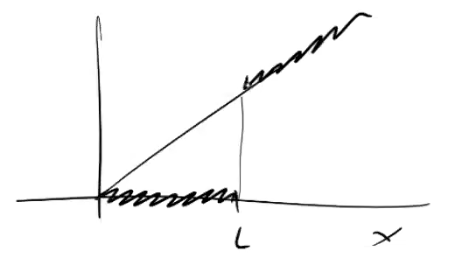
\includegraphics[scale=0.3]{fig/tmp/fig39}
  \caption{Graphical representation of $ST_L(x)$.}
\end{figure}
We now turn to a more interesting example, which is quoted in the market: the \textbf{down-and-out European call} (DOC) with strike price $K$. The payoff of this contract is given by
\begin{equation}
  \pay_T(\text{DOC}) = (S(T)-K)^+\,\mathds{1}_{S(t)>L,\forall t\in[0,T]}
\end{equation}
In order to price this contract we have to consider the modified payoff
\begin{equation}
  (S(T)-K)^+\,\mathds{1}_{S(T)>L} = (S(T)-K)\mathds{1}_{S(T)>K}\mathds{1}_{S(T)>L}
\end{equation}
According to the possible values of $L$ and $K$ we have different situations:
\begin{itemize}
  \item if $K>L$ then the indicator function $\mathds{1}_{S(t)>L}$ is redundant and the modification of the payoff coincides with the original payoff. However, even if the modification of the payoff coincides with the original payoff, we cannot say that the barrier option price coincides with the vanilla call option price, as we will see.
  \item if $K>L$ then we can exercise the contract but due to the presence of the indicator function of $L$ the terminal payoff can be different. In this case the indicator function $\mathds{1}_{S(t)>K}$ is redundant and the modified payoff is given by
  \begin{equation*}
    (S(T)-K)\mathds{1}_{S(T)>L}
  \end{equation*}
  This can be seen as the payoff of a combination of a call option and a digital option. In fact, we can write
  \begin{align*}
    (S(T)-K)\mathds{1}_{S(T)>L} &= (S(T)-L+L-K)\mathds{1}_{S(T)>L} \\
    &=
    (S(T)-L)^+ + (L-K)\mathds{1}_{S(T)>L}
  \end{align*}
\end{itemize}
The result for the pricing function in these two cases is as follows.
\begin{proposition}[Down-and-out call pricing]
  The down-and-out European call option is priced as follows. For $L<K$:
  \begin{equation}\label{clo}
    C_{LO}(t,s,K) = \left[C(t,s,K)-\left(\frac{L}{s}\right)^{\left(\frac{2\Tilde{r}}{\sigma^2}\right)} C\left(t,\frac{L^2}{s},K\right)\right]\mathds{1}_{s>L}.
  \end{equation}
  For $L>K$:
  \begin{align}
      \notag C_{LO}(t,s,K) &= \bigg\{C(t,s,K) + (L-K)H(t,s,L) - \\
      &\qquad
      - \left(\frac{L}{s}\right)^{\left(\frac{2\Tilde{r}}{\sigma^2}\right)}
      \left[C\left(t,\frac{L^2}{s},K\right) + (L-K)H\left(t,\frac{L^2}{s},K\right)\right]\bigg\}\mathds{1}_{s>L}
  \end{align}
\end{proposition}
In Section \ref{putcallparity} we used this linearity to prove the standard put–call parity relation for standard European options, and we can now derive the put–call parity result for down-and-out options, often called \textbf{DOC-DOP parity}. Recall that the payoff of a put option is given by
\begin{align*}
    P(x,K) = (K-x)^+ &= K - x - (x - K)^+ \\
    &=
    K\cdot BO(x) - ST(x) + C(x,K)
\end{align*}
Using Corollary \ref{linearitycor} we immediately have the following result.
\begin{proposition}[Down-and-out put pricing]
    The down-and-out put price $P_{LO}$, and call price $C_{LO}$, are related by the formula
    \begin{equation}
        P_{LO}(t, s, K) = K\cdot B_{LO}(t, s) - ST_{LO}(t,s) + C_{LO}(t, s, K).
    \end{equation}
\end{proposition}
Note that when $L = 0$ we have the usual put–call parity.\\
We now want to compute the price of a European \textbf{up-and-out put option} (UOP) with barrier $L$ and strike price $K$. As usual, we have to consider a modification of the payoff:
\begin{equation}
    P^L(x,K)=(K-x)+\mathds{1}_{x<L} = (K-x)\mathds{1}_{x<K}\mathds{1}_{x<L}
\end{equation}
There are two possibilities:
\begin{itemize}
    \item if $L > K$ then the indicator function $\mathds{1}_{x<L}$ is redundant and the modification of the payoff is the same of the vanilla put:
    \begin{equation*}
        P^L(x, K) = (K - x)^+
    \end{equation*}
    Again, this does not mean that the price of this barrier option is the same of the vanilla put option.
    \item if $L < K$ then the indicator function $\mathds{1}_{x<K}$ is redundant and the modification of the payoff is given by
    \begin{align*}
        P^L(x, K) &= (K-x)\mathds{1}_{x<L} =(L-x)\mathds{1}_{x<L}+(K-L)\mathds{1}_{x<L} \\
        &=
        (L-x)^+ +(K-L)-(K-L)\mathds{1}_{x<L}
    \end{align*}
    which is the combination of the payoff of a put option and two digital options.
\end{itemize}
Now we know how to price every building block of the up-and-out, so we can give the pricing function.
\begin{proposition}[Up-and-out put pricing]
    The price of an up-and-out European put option is given by the following formulas. For $L > K$:
    \begin{equation}
      P^{LO}(t,s,K) = \left[P(t,s,K)-\left(\frac{L}{s}\right)^{\left(\frac{2\Tilde{r}}{\sigma^2}\right)} P\left(t,\frac{L^2}{s},K\right)\right]\mathds{1}_{s<L}.
    \end{equation}
    For $L>K$:
    \begin{align}
        \notag P^{LO}(t,s,K) &= \bigg\{P(t,s,L) + (K-L)H(t,s,L) - \\
        &\qquad
        \notag - \left(\frac{L}{s}\right)^{\left(\frac{2\Tilde{r}}{\sigma^2}\right)}
        \left[P\left(t,\frac{L^2}{s},L\right) - (K-L) H\left(t,\frac{L^2}{s},L\right)\right] +\\
        &\qquad
        \left[1-\left(\frac{L}{s}\right)^{\left(\frac{2\Tilde{r}}{\sigma^2}\right)}\right] (K-L)e^{-r(T-t)}\bigg\}\mathds{1}_{s>L}.
    \end{align}
\end{proposition}
In order to price a \textbf{up-and-out call option} (UOC) we can use the put-call parity. Alternatively, if we use the ``direct approach", we have to consider the payoff modification
\begin{align*}
    (S-K)^+\mathds{1}_{s<L} &= (S-K)^+\mathds{1}_{s<L} \\
    &=
    (S-K)\mathds{1}_{s>K}(1-\mathds{1}_{s>L}) \\
    &=
    (S-K)^+ - (S-K)\mathds{1}_{s>K}\mathds{1}_{s>L}
\end{align*}
and then consider the different cases. \colorbox{cyan}{homework}

\subsubsection{Knock-in contracts}
Knock-in contracts are contracts which will start to exist if and only if the price of the underlying stock hits a prespecified barrier level at some time during the contract period. We thus fix a standard $T$-claim of the form $Z = \Phi(S(T))$, and we also fix a barrier $L$. \\
We start by studying the \textbf{down-and-in} version of $Z$, which is defined as follows:
\begin{equation}
    Z_{LI} =
    \begin{cases}
        0 & \text{if } S(t)>L\,\,\forall t\in[0,T] \\
        \Phi(S(T)) & \text{otherwise}
    \end{cases}
\end{equation}
$L$ as a subscript indicates a ``down" contract, whereas the subscript $I$ denotes a ``in" contract. Pricing a down-and-in contract turns out to be fairly easy, since we can in fact price it in terms of the corresponding down-and-out contract.
\begin{lemma}[In-out parity]
    $F_{LI}(t, s, \Phi) = F(t, s, \Phi) - F_{LO}(t, s, \Phi),\,\, \forall s$.
\end{lemma}
\begin{proof}
    If, at time $t$, we have a portfolio consisting of a down-and-out version of $Z$ as well as a down-and-in version of $Z$ (with the same barrier $L$) then
    \begin{equation*}
        Z_{LI} + Z_{LO} = \Phi,
    \end{equation*}
    so we wil receive exactly $Z$ at time $T$. We thus have
    \begin{equation*}
        F_{LI} (t, s, \Phi) = F(t, s, \Phi) - F_{LO}(t, s, \Phi).
    \end{equation*}
\end{proof}
We can now formulate the basic result.
\begin{proposition}[Down-and-in pricing]
    Consider a fixed $T$-contract $Z = \Phi(S(T))$. Then the price of the corresponding down-and-in contract $Z_{LI}$ is given by
    \begin{equation}
        F_{LI}(t,s,\Phi) = \left[F(t,s,\Phi^L)-\left(\frac{L}{s}\right)^{\left(\frac{2\Tilde{r}}{\sigma^2}\right)} F\left(t,\frac{L^2}{s},\Phi^L\right)\right]\mathds{1}_{s<L}.
    \end{equation}
\end{proposition}
\begin{proof}
    From the equality $\Phi_L + \Phi^L = \Phi$ we have
    \begin{align*}
        F_{LI}(t,s,\Phi) &= F(t,s,\Phi) + F_{LO}(t,s,\Phi) \\
        \overset{\ref{clo}}&{=}
        \cancel{F(t,s,\Phi_L)} + F(t,s,\Phi^L) - \left[\cancel{F(t,s,\Phi_L)} - \left(\frac{L}{s}\right)^{\left(\frac{2\Tilde{r}}{\sigma^2}\right)} F(t,s,\Phi_L)\right] \\
        &=
        \left[F(t,s,\Phi^L) - \left(\frac{L}{s}\right)^{\left(\frac{2\Tilde{r}}{\sigma^2}\right)} F\left(t,\frac{L^2}{s},\Phi^L\right)\right].
    \end{align*}
\end{proof}
The treatment of up-and-in contracts is of course parallel to down-and-in contracts.
\begin{proposition}[Up-and-in pricing]
    Consider a fixed $T$-contract $Z = \Phi(S(T))$. Then the price of the corresponding up-and-in contract $Z^{LI}$ is given by
    \begin{equation}
        F^{LI}(t,s,\Phi) = \left[F(t,s,\Phi_L) - \left(\frac{L}{s}\right)^{\left(\frac{2\Tilde{r}}{\sigma^2}\right)} F\left(t,\frac{L^2}{s},\Phi_L\right)\right]\mathds{1}_{s<L}.
    \end{equation}
\end{proposition}
\begin{proof}
    Same argument as before.
\end{proof}
As an example, we give the pricing formula for a \textbf{down-and-in European call} with strike price $K$.
\begin{proposition}[Down-and-in call pricing]
    For $s > L$ the down-and-in European call option is priced as follows. For $L<K$
    \begin{equation}
        C_{LI}(t,s,\Phi) = \left(\frac{L}{s}\right)^{\left(\frac{2\Tilde{r}}{\sigma^2}\right)} C\left(t,\frac{L^2}{s},K\right).
    \end{equation}
    For $L>K$:
    \begin{equation}
        C_{LI}(t,s,\Phi) = \left(\frac{L}{s}\right)^{\left(\frac{2\Tilde{r}}{\sigma^2}\right)} \left[C\left(t,\frac{L^2}{s},K\right) + (L-K)H\left(t,\frac{L^2}{s},L\right)\right] - (L-K)H(t,s,L).
    \end{equation}
\end{proposition}

\subsubsection{Lookbacks}
Lookback options are contracts which at the delivery time $T$ allow us to take advantage of the realized maximum or minimum of the underlying price process over the entire contract period. Typical examples are:
\begin{align*}
    \Phi(T) = (S(T)-\min_{t\le T}S(t)) \qquad &\text{Lookback call} \\
    \Phi(T) = \max_{t\le T}S(t) - S(t) \qquad &\text{Lookback put} \\
    \Phi(T) = \left(\max_{t\le T}S(t) - K\right)^+ \qquad &\text{Forward lookback call} \\
    \Phi(T) = \left(K-\min_{t\le T}S(t)\right)^+ \qquad &\text{Forward lookback put}
\end{align*}
In order to price this kind of contracts, we need the distribution of the maximum
\begin{equation}
    M_S(t) = \max_{t\le T} S(t)
\end{equation}
and of the minimum
\begin{equation}
    m_S(t) = \min_{t\le T} S(t)
\end{equation}
Recall that
\begin{equation*}
    S(t) = e^{\ln s + \tilde{r} t + \sigma W(t)} = e^{X(t)}
\end{equation*}
where
\begin{equation*}
    \begin{cases}
        \dd X(t) = \tilde{r}\,\dd t + \sigma\,\dd W(t) \\
        X(0) = \ln s
    \end{cases}
\end{equation*}
Therefore
\begin{equation*}
    M_S(t) = e^{M_X(t)}
\end{equation*}
The distribution for $M_X(T)$ is known to us from Proposition \ref{f}. Thanks to this proposition we obtain the distribution function, $F$, for $M_X(T)$:
\begin{equation}
    F_{\max_{s\le t}X_s}(x) = \left[
    \varphi\left(\frac{x-\alpha-\mu t}{\sigma\sqrt{t}}\right)
    -\exp{-\frac{2\mu(\alpha-\beta)}{\sigma^2}}\varphi\left(-\frac{x-\alpha+\mu t}{\sigma\sqrt{t}}\right)
    \right]\mathds{1}_{x\ge\ln s}
\end{equation}
From this expression we can compute the density function $f=F'$ and then the expected value
\begin{equation}
    \expect\left[\max_{t\le T}S(t)\right] = \expect\left[e^{M_X(T)}\right] = \int_{\ln s}^{\infty}e^x f(x)\,\dd x
\end{equation}
After a series of elementary, but extremely tedious, partial integrations we end up with the following result.
\begin{proposition}
    The price, at $t=0$, of the lookback put is given by
    \begin{equation}
        price_0(\mbox{\emph{lookback put}}) = -s\varphi(-d) + se^{-rT}\varphi\left(-d+\sigma\sqrt{T}\right)\left(1-\frac{\sigma^2}{2r}+ \frac{s\sigma^2}{2r}N(d)\right)
    \end{equation}
    where
    \begin{equation}
        d = \frac{rT + \tfrac{1}{2}\sigma^2 T}{\sigma\sqrt{T}}.
    \end{equation}
\end{proposition}
